\section{Introduction}

Recently, Linux containers have drawn a significant amount of attention because they are lightweight, portable, and reproducible.
Linux containers are generally more lightweight than virtual machine (VM), because the containers share the kernel with the host operating system (OS), even though they maintain separate execution environments.
They are generally portable because the process execution environments are archived into tar files,
so whenever one attempts to run a container, the exact same file systems are restored from the archives
even when totally different data centers are used.
This means that containers can provide reproducible and portable execution environments.
%
For the same reasons, Linux containers are attractive for web services as well,
and it is expected that web services consisting of container clusters would be
capable of being migrated easily for a variety of purposes. For example disaster recovery,
cost performance improvements, legal compliance, and shortening the geographical distance to customers
are the main concerns for web service providers in e-commerce, gaming, Financial technology(Fintech) and Internet of Things(IoT) field.
%

Kubernetes\cite{K8s2017}, which is one of the most popular container cluster management systems, 
enables easy deployment of container clusters.
Since Kubernetes seems to hide the differences in the base environments, users are expected to be able to easily deploy a web service on different 
cloud providers or on on-premise data centers, without adjusting the container cluster configurations to the new environment. 
This allows a user to easily migrate a web service consisting of a container cluster even to the other side of the world as follows: 
A user starts the container cluster in the new location, route the traffic there, 
then stop the old container cluster at his or her convenience.
This is a typical web service migration scenario.

However, this scenario only works when the user migrates a container cluster among major cloud providers including Google Cloud Platform (GCP), 
Amazon Web Services (AWS), and Microsoft Azure.
Kubernetes does not provide generic ways to route the traffic from the internet into container cluster running in the Kubernetes and is 
heavily dependent on cloud load balancers, which is external load balancers that are set up on the fly by cloud providers through their application protocol interfaces (APIs).
%
These cloud load balancers distribute incoming traffic to every server that hosts containers.
The traffic is then distributed again to destination containers using iptables destination 
network address translation (DNAT)\cite{MartinA.Brown2017,Marmol2015} rules in a round-robin manner. 
The problem happens in the environment with a load balancer that is not supported by the Kubernetes, 
e.g. in an on-premise data center with a bare metal load balancer. 
In such environments, the user needs to manually configure 
the static route for inbound traffic in an ad-hoc manner. 
Since the Kubernetes fails to provide a uniform environment from a container cluster viewpoint,
migrating container clusters among the different environments will always be a burden.

In order to solve this problem by eliminating the dependency on cloud load balancers,
we have proposed a containerized software load balancer that is run by Kubernetes as  
a part of web service container clusters in the previous work\cite{takahashi2018portable}.
It enables a user to deploy a web service in different environments without modification because the web service itself includes load balancers.
%
We containerized Linux kernel's Internet Protocol Virtual Server (IPVS)\cite{Zhang2000} 
Layer 4 load balancer using an existing Kubernetes ingress\cite{K8sIngress2017} framework, as a proof of concept.
%
%
We also proved that our approach does not significantly degrade the performance,
by comparing the performance of our proposed load balancer with those of
iptables DNAT load balancer and the Nginx Layer 7 load balancing.
%
The results indicated that the proposed load balancer could improve the portability of container clusters without performance degradation compared with the existing load balancer.

However, the way to route traffic from the Internet to load balancers while keeping redundancy has not been discussed in our previous work, even though the redundancy is always needed to improve the availability of services in modern systems.
This is because, standard Layer 2 redundancy protocols, e.g., Virtual Router Redundancy Protocol(VRRP)\cite{hinden2004virtual}
or OSPF\cite{moy1997ospf}, which uses multicast, cannot be used in many network environments for containers.
Furthermore, providing uniform methods independent of the infrastructures such as various cloud environments and the on-premise data center is much more difficult.

In this paper, we extend the previous work and propose a software load balancer architecture with Equal Cost Multi-Path(ECMP)\cite{thaler2000multipath} redundancy by running a Border Gateway Protocol(BGP) agent container together with ipvs container.
In order to demonstrate the feasibility of the proposed load balancer, we containerize an open source BGP software, exabgp\cite{exa-networks_2018}, and also containerize Linux kernel's ipvs load balancer. Then we launch them as a single pod, which is a group of containers that share a single net namespace using Kubernetes. We launch multiple of such pods and form a cluster of load balancers.
We demonstrate the functionality and evaluate preliminary performance.

The contributions of this paper are as follows:
Although there have been studies regarding redundant software load balancers especially from the major cloud providers\cite{eisenbud2016maglev,patel2013ananta}, their load balancers are only usable within their respective cloud infrastructures.
This paper aims to provide a redundant software load balancer architecture for those environments that do not have load balancers supported by Kubernetes.
Since proposed load balancer architecture uses nothing but existing Open Source Software(OSS) and standard Linux boxes, users can build a cluster of redundant load balancers in their environment.

The rest of the paper is organized as follows.
Section \ref{Related Work} highlights related work.
Section \ref{Proposed Architecture} discusses problems of the existing architecture and proposes our solutions.
In Section \ref{Implementation}, we explain experimental system in detail.
Then, we show our experimental results and discuss obtained characteristics in Section~\ref{Evaluation}, which is followed by a summary of our work in Section~\ref{Conclusions}.

\section{Related Work}\label{Related Work}

This section highlights related work, especially that dealing with container cluster migration, 
software load balancer containerization, load balancer tools within the context of the container technology and scalable load balancer in the cloud providers.

\paragraph{\bf Container cluster migration:}

Kubernetes developers are trying to add federation\cite{K8sFederation2017} capability for handling situations 
where multiple Kubernetes clusters\footnote{The {\em Kubernetes cluster} refers to a server cluster 
controlled by the Kubernetes container management system, in this paper.} 
are deployed on multiple cloud providers or on-premise data centers, 
and are managed via the Kubernetes federation API server (federation-apiserver). 
However, how each Kubernetes cluster is run on different types of cloud providers
and/or on-premise data centers, especially when the load balancers of such environments are not supported by Kubernetes, 
seems beyond the scope of that project. 
The main scope of this paper is to make Kubernetes usable in environments 
without supported load balancers by providing a containerized software load balancer.

\paragraph{\bf Software load balancer containerization:}
As far as load balancer containerization is concerned, the following related work has been identified:
Nginx-ingress\cite{Pleshakov2016,NginxInc2016} utilizes the ingress\cite{K8sIngress2017} capability of Kubernetes, 
to implement a containerized Nginx proxy as a load balancer. Nginx itself is famous as a high-performance web server program
that also has the functionality of a Layer-7 load balancer. Nginx is capable of handling Transport Layer Security(TLS) encryption, 
as well as Uniform Resource Identifier(URI) based switching. However, the flip side of Nginx is that it is much slower than Layer-4 switching.
We compared the performance between Nginx as a load balancer and our proposed load balancer in this paper.
%
Meanwhile, the kube-keepalived-vip\cite{Prashanth2016} project is trying to use Linux kernel's ipvs\cite{Zhang2000} 
load balancer capabilities by containerizing the keepalived\cite{ACassen2016}.
The kernel ipvs function is set up in the host OS's net namespaces and is shared among multiple web services,
as if it is part of the Kubernetes cluster infrastructure.
Our approach differs in that the ipvs rules are set up in container's net namespaces 
and function as a part of the web service container cluster itself.
The load balancers are configurable one by one, and are  movable with the cluster once the migration is needed.
The kube-keepalived-vip's approach lacks flexibility and portability whereas ours provide them.
%
The swarm mode of the Docker\cite{DockerCoreEngineering2016,DockerInc2017} also uses ipvs for internal load balancing,
but it is also considered as part of Docker swarm infrastructure, 
and thus lacks the portability that our proposal aims to provide.

\paragraph{\bf Load balancer tools in the container context:}
There are several other projects where efforts have been made to utilize ipvs in the context of container environment.
For example, GORB\cite{Sibiryov2015} and clusterf\cite{Aaltodoc:http://urn.fi/URN:NBN:fi:aalto-201611025433} are daemons 
that setup ipvs rules in the kernel inside the Docker container. 
They utilize running container information stored in key-value storages
like Core OS etcd\cite{CoreOSEtcd} and HashiCorp's Consul\cite{HashiCorpConsul}. 
Although these were usable to implement a containerized load balancer in our proposal, we did not use them, 
since Kubernetes ingress framework already provided the methods to retrieve running container information through standard API.

\paragraph{\bf Cloud load balancers:}

As far as the cloud load balancers are concerned, two articles have been identified.
Google's Maglev\cite{eisenbud2016maglev} is a software load balancer used in Google Cloud Platform(GCP).
Maglev uses modern technologies including per flow ECMP and kernel bypass for user space packet processing.
Maglev serves as the GCP's load balancer that is used by the Kubernetes.
Maglev is not a product that users can use outside of GCP nor is an open source software, while the users need open source software load balancer that is runnable even in on-premise data centers.
Microsoft's Ananta\cite{patel2013ananta} is another software load balancer implementation using ECMP and windows network stack.
Ananta can be solely used in Microsoft's Azure cloud infrastructure\cite{patel2013ananta}.
The proposed load balancer by the author is different in that it is aimed to be used in every cloud provider and on-premise data centers.

\section{Proposed Architecture}\label{Proposed Architecture}

Here we discuss a general overview of the proposed load balancer architectures.

%\subsection{A containerized Load balancer}

\subsection{Problems of Kubernetes Cluster}

\begin{figure}[tb]
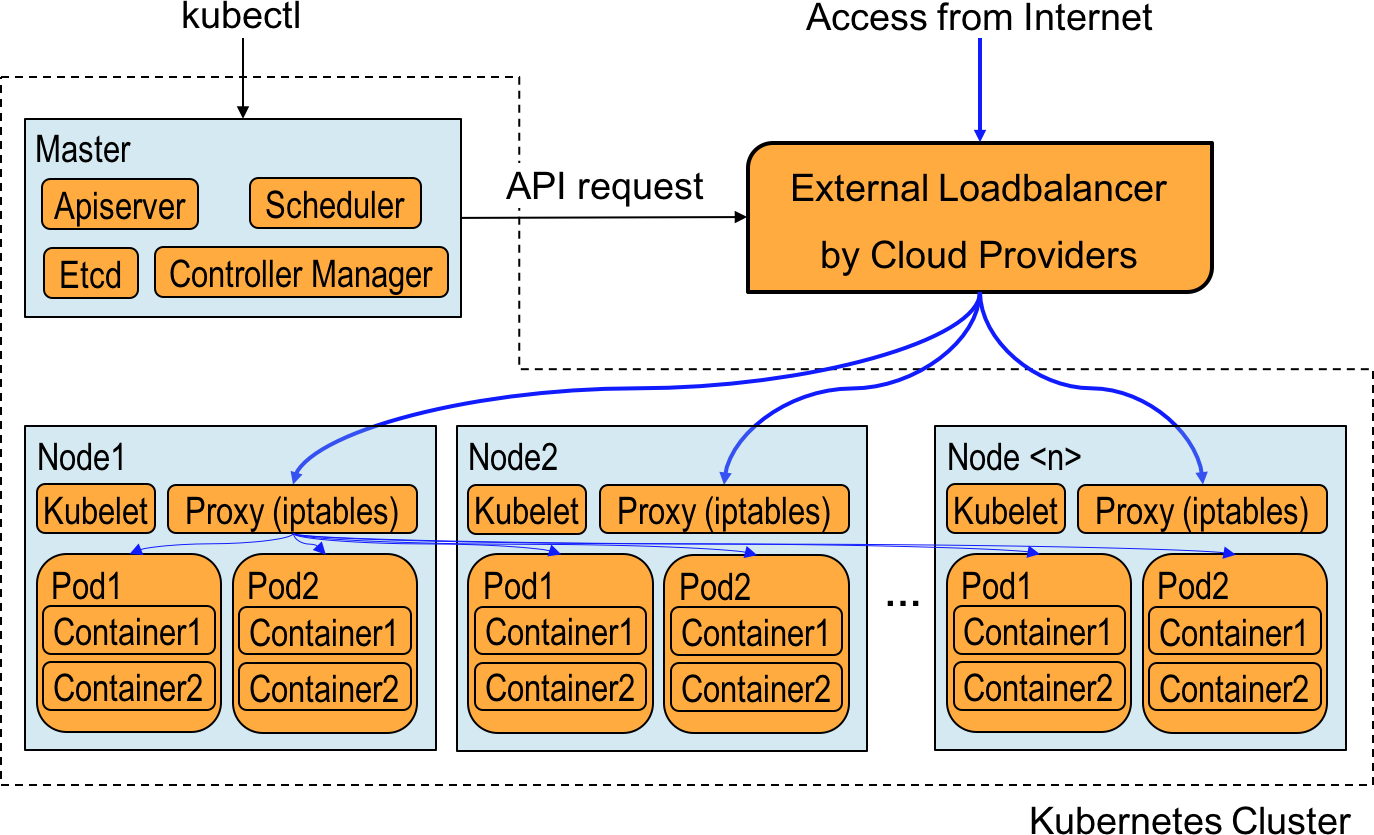
\includegraphics[width=\columnwidth]{Figs/K8sConventional}
\caption{Conventional architecture of a Kubernetes cluster.}
\textcolor{blue}{
  Kubernetes is dependent on external cloud load balancers.
This is a problem since bare metal load balancers in on-premise data centers are most likely not supported by Kubernetes.
}
\label{fig:K8sConventional}
\end{figure}

Problems commonly occur when the Kubernetes container management system is used outside of recommended cloud providers(such as GCP or AWS).
Figure~\ref{fig:K8sConventional} shows an exemplified Kubernetes cluster.
A Kubernetes cluster typically consists of a master and nodes. They can be physical servers or VMs.
On the master, daemons that control the Kubernetes cluster are typically deployed. 
These daemons include, Apiserver, Scheduler, Controller-manager and Etcd. 
On the nodes, kubelet and proxy daemons are running.
The kubelet daemon will run {\it pods}, depending the PodSpec information obtained from the apiserver on the master.
A {\em pod} is a group of containers that share same net namespace and cgroups, 
and is the basic execution unit in a Kubernetes cluster.

When a service is created, the master will schedule where to run {\em pods} and kubelets on the nodes will launch them accordingly.
At the same time, the masters will send out requests to cloud provider API endpoints, asking them to set up external cloud load balancers.
The proxy daemon on the nodes will also setup iptables DNAT\cite{MartinA.Brown2017} rules. 
The Internet traffic will then be evenly distributed by the cloud load balancer to nodes, 
after which it will be distributed again by the DNAT rules on the nodes to the designated {\em pods}. 
The returning packets will follow the exact same route as the incoming ones.

This architecture has the followings problems: 
1) Having cloud load balancers whose APIs are supported by the Kubernetes daemons is a prerequisite.
There are numerous load balancers that are not supported by the Kubernetes.
These include the bare metal load balancers for on-premise data centers.
In such cases, users are required to set up the routing manually depending on the infrastructure.
However, this approach significantly degrades the portability of container clusters.
2) Distributing the traffic twice, first on the external load balancers and second on each node, 
complicates the administration of packet routing. 
Imagine a situation in which the DNAT table on one of the nodes malfunctions.
In such a case, only occasional timeouts would be observed, which would make it very difficult to find out which node was malfunctioning.   

In short, 1) Kubernetes is optimized only for limited environments where the external load balancers are supported, 
and 2) the routes incoming traffic follow are very complex.
%
To address these problems, we propose a containerized software load balancer with ECMP redundancy for environments without a cloud load balancer.

\begin{figure}[tb]
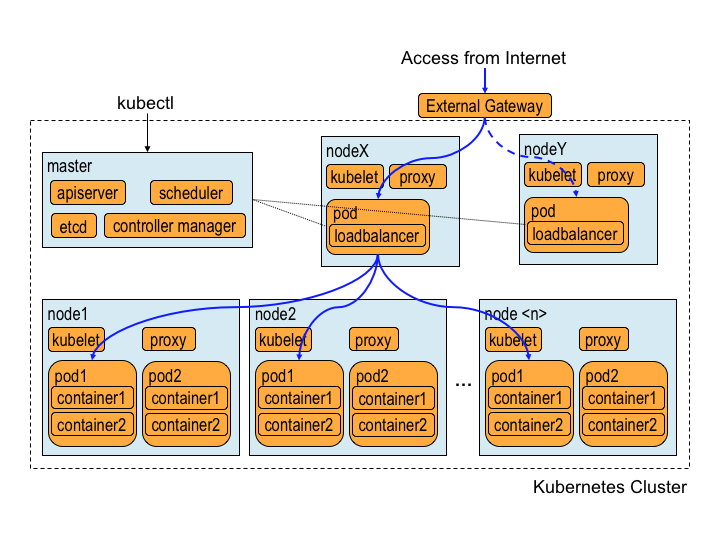
\includegraphics[width=1.0\columnwidth]{Figs/K8sProposed}
\caption{Kubernetes cluster with proposed load balancer.}
The proposed architecture includes software load balancers in container cluster itself thereby removing the dependency on external cloud load balancers.
\label{fig:K8sProposed}
\end{figure}

\subsection{Proposed architecture: a portable load balancer}

Figure~\ref{fig:K8sProposed} shows the proposed  Kubernetes cluster architecture, 
which has the following characteristics:
1) Each load balancer itself is run as a {\em pod} by Kubernetes. 
2) Load balancer configurations are dynamically updated based on information about running {\em pods}.
%%3) There exist multiple load balancers for redundancy. 
The proposed load balancer can resolve the conventional architecture problems, as follows:
Since the load balancer itself is containerized, the load balancer can run in any environment including on-premise data centers, 
even without external load balancers that is supported by Kubernetes.
The incoming traffic is directly distributed to designated {\em pods} by the load balancer. 
It makes the administration, e.g. finding malfunctions, easier.

We designed the proposed load balancer using three components, ipvs, keepalived, and a controller. 
These components are placed in a Docker container image.
The ipvs is a Layer-4 load balancer capability, which is included in the Linux kernel 2.6.0 released in 2003 or later, 
to distribute incoming Transmission Control Protocol(TCP) traffic to 
{\em real servers}\footnote{The term, {\em real servers} refers to worker servers that will respond to incoming traffic, 
in the original literature\cite{Zhang2000}. We will also use this term in the similar way.}\cite{Zhang2000}. 
For example, ipvs distributes incoming Hypertext Transfer Protocol(HTTP) traffic destined for a single destination IP address, 
to multiple HTTP servers(e.g. Apache HTTP or nginx) running on multiple nodes in order to improve the performance of web services.
Keepalived is a management program that performs health checking for {\em real servers}
and manages ipvs balancing rules in the kernel accordingly.
It is often used together with ipvs to facilitate ease of use.
The controller is a daemon that periodically monitors the {\em pod} information on the master, 
and it performs various actions when such information changes.
Kubernetes provides ingress controller framework as the Go Language(Golang) package to implement the controllers. 
We have implemented a controller program that feeds {\em pod} state changes to keepalived 
using this framework. 

\subsection{Proposed architecture: load balancer redundancy}

While containerizing ipvs makes it runnable in any environment, it is essential to discuss how to route the traffic to the ipvs container.
We propose redundant architecture using ECMP with BGP for load balancer containers usable especially in on-premise data centers.
We first explain overlay network briefly to understand requirements for the architecture in \ref{Overlay network}, then present the proposed architecture with ECMP redundancy in \ref{Redundancy with ECMP}. 
\textcolor{blue}{
(As a complement, we also present an alternative architecture using VRRP for a comparison in \ref{appendix:Redundancy with VRRP}, which we think is not as good as the architecture using ECMP.)
}

\textcolor{blue}{
Although major cloud providers do not currently provide BGP peering service for their users, the authors expect they start such service, once this approach is proven to be beneficial.
Therefore we focus our discussions on verifying that our proposed load balancer architecture is feasible at least in on-premise data centers.
For the cloud environment without BGP peering service, we can still launch our proposed load balancer without ECMP redundancy by sending out API request to automatically set up a route to the load balancer, from inside the ipvs container.
}

\paragraph{\bf Overlay network}\label{Overlay network}

In order to discuss load balancer redundancy, the knowledge of the overlay network is essential.
We briefly explain an abstract concept of overlay network that is common to existing overlay network including flannel\cite{coreos_2018} and calico\cite{project_calico}.

\begin{figure}[tb]
\begin{center}
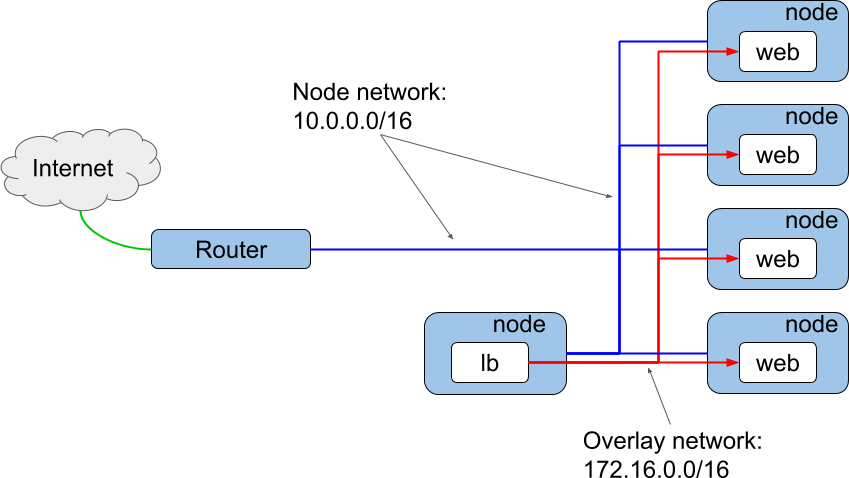
\includegraphics[width=\columnwidth]{Figs/overlay.png}
\end{center}
\caption{The network architecture of an exemplified container cluster system.}
A load balancer(lb) pod(the white box with "lb") and web pods are running on nodes(the blue boxes).
  The traffic from the internet are forwarded to the lb pod by the upstream router using the node network,
  and the distributed to web pods using the overlay network.
\label{fig:overlay}
\end{figure}

Fig.~\ref{fig:overlay} shows schematic diagram of network architecture of a container cluster system. 
Suppose we have a physical network(node network) with IP address range of 10.0.0.0/16 and an overlay network with IP address range of 172.16.0.0/16.
The node network is the network for nodes to communicate with each other.
The overlay network is the network setups for containers to communicate with each other.
An overlay network typically consists of appropriate routing tables on nodes, and optionally of tunneling setup using ipip or vxlan.
The upstream router usually belongs to the node network.
When a container in the Fig.~\ref{fig:overlay} communicates with any of the nodes, it can use its IP address in 172.16.0.0/16 IP range as a source IP, since every node has proper routing table for the overlay network.
When a container communicates with the upstream router that does not have routing information regarding the overlay network, the source IP address must be translated by Source Network Address Translation(SNAT) rules on the node the container resides.

The SNAT caused a problem when we tried to co-host multiple load balancer pods for different services on a single node and let them connect the upstream router directly.
This was due to the fact that the BGP agent used in our experiment only used the source IP address of the connection to distinguish the BGP peer.
The agent behaved as though different BGP connections from different containers belonged to a single BGP session because the source IP addresses were identical due to the SNAT.
We propose the architecture that solves this problem in (2).

\paragraph{\bf Redundancy with ECMP}\label{Redundancy with ECMP}

\begin{figure}[tb]
\begin{center}
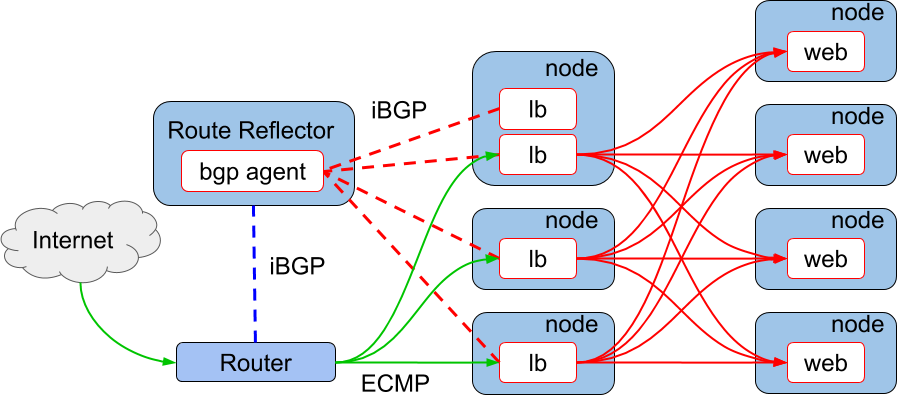
\includegraphics[width=\columnwidth]{Figs/ecmp.png}
\end{center}
\caption{The proposed architecture of load balancer redundancy with ECMP.}
\textcolor{blue}{
  The traffic from the internet is distributed by the upstream router to multiple of lb pods using hash-based ECMP(the solid green line) and then distributed by the lb pods to web pods using Linux kernel's ipvs(the solid red line).
  The route to an IP address for a service(we call this address, service IP) is advertised to the route reflector(the dotted red line) and then advertised to the upstream router(the blue dotted line) using iBGP.
  For the green lines, a service IP address is used. The red lines use the IP addresses of the overlay network. The blue line uses the IP addresses of the node network.
}
\label{fig:ecmp}
\end{figure}

Fig.~\ref{fig:ecmp} shows our proposed redundancy architecture with ECMP for software load balancer containers.
%
The ECMP is a functionality a router often supports, where the router has multiple next hops with equal cost(priority) to a destination, and generally distribute the traffic depending on the hash of the flow five tuples(source IP, destination IP, source port, destination port, protocol).
The multiple next hops and their cost are often populated using the BGP protocol.
%
The notable benefit of the ECMP setup is the fact that it is scalable.
All the load balancers that claims as the next hop is active, i.e., all of them are utilized to increase the performance level.
Since the traffic from the internet is distributed by the upstream router, the overall throughput is determined by the router after all.
However, in practice, there are a lot of cases where this architecture is beneficial.
For example, if a software load balancer is capable of handling 1 Gbps equivalent of traffic and the upstream router is capable of handling 10 Gbps, it still is worthwhile launching 10 of the software load balancer containers to fill up maximum throughput of the upstream router.

%
We place a node with the knowledge of the overlay network as a route reflector, to deal with the complexity due to the SNAT described in (1).
A route reflector is a network component for BGP to reduce the number of peerings by aggregating the routing information\cite{rfc4456}.
In our proposed architecture we use it as a delegater for load balancer containers towards the upstream router.

By using the route reflector, we can have the following benefits.
1) Each node can accommodate multiple load balancer containers. This was not possible when we tried to directly connect load balancers and the router through SNAT.
2) The router does not need to allow peering connections from random IP addresses that may be used by load balancer containers. Now, the router only need to have the reflector information as the BGP peer definition.

Since we use standard Linux boxes for route reflectors, we can configure them as we like;
a) We can make them belong to overlay network so that multiple BGP sessions from a single node can be established.
b) We can use a BGP agent that supports dynamic neighbor (or dynamic peer), where one only needs to define the IP range as a peer group and does away with specifying every possible IP that load balancers may use.

The upstream router does not need to accept BGP sessions from containers with random IP addresses, but only from the router reflector with well known fixed IP address. This may be preferable in terms of security especially when a different organization administers the upstream router.
Although not shown in the Fig.~\ref{fig:ecmp}, we could also place another route reflector for redundancy purpose.


\section{Implementation}\label{Implementation}

Here we discuss the implementation of the experimental system to prove the concept of our proposed load balancers with ECMP redundancy in detail.

\subsection{Experimental system architecture}

\begin{figure}[tb]
\begin{center}
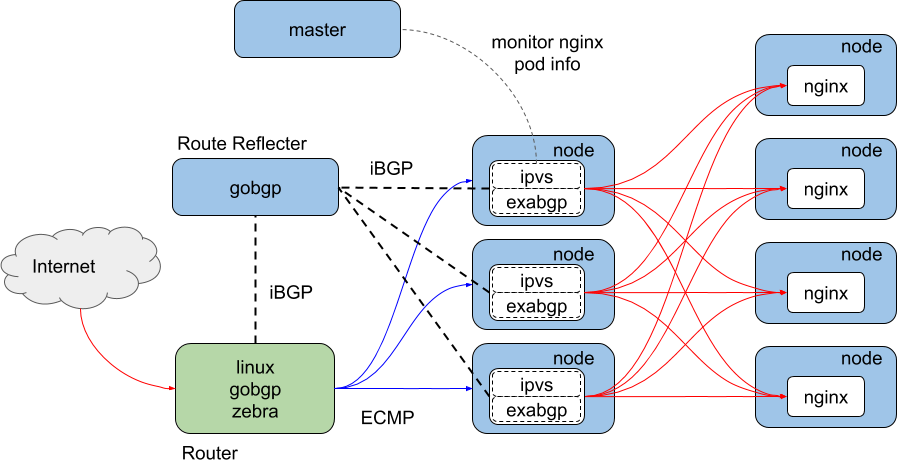
\includegraphics[width=\columnwidth]{Figs/poc.png}
\end{center}
\caption{An experimental container cluster with proposed redundant software balancers. }
  The master and nodes are configured as Kubernetes's master and nodes on top of conventional Linux boxes, respectively.
  The route reflector and the upstream router are also conventional Linux boxes.
\textcolor{blue}{
  For the green lines, a service IP address is used. The red lines use the IP addresses of the overlay network. The blue line uses the IP addresses of the node network.
}
\label{fig:poc}
\end{figure}

Fig.~\ref{fig:poc} shows the schematic diagram of proof of concept container cluster system with our proposed redundant software load balancers.
All the nodes and route reflector are configured using Debian 9.5 with self compiled linux-4.16.12 kernel.  
We also used a conventional Linux box with the same OS for the upstream router.
For the Linux kernel to support hash based ECMP routing table we needed to use kernel version 4.12 or later.
We also needed to enable kernel configuration option CONFIG\_IP\_ROUTE\_MULTIPATH\cite{ip-sysctl} when compiling, and set the kernel parameter fib\_multipath\_hash\_policy=1 at run time.
In the actual production environment, proprietary hardware with the highest throughput is often used for the upstream router, but we could still test some of the required advanced functions by using a Linux box.

Each load balancer pod consists of an exabgp container and an ipvs container.
The ipvs container is responsible for distributing the traffic destined to an IP address that a service uses(service IPs) toward web(nginx) server pods.
The IP address for nginx pods and load balancer pods are dynamically assigned upon launch of themselves from 172.16.0.0/16 address range.
The ipvs container monitors the availability of web server pods and manages the load balancing rule appropriately.
The exabgp container is responsible for advertising the route toward the service IP to the route reflector.
The route reflector aggregates the routing information advertised by load balancer pods and advertise them to the upstream router.

Exabgp is used in the load balancer pods because of the simplicity in setting as static route advertiser.
On the other hand, gobgp is used in the router and the route reflector, because exabgp did not seem to support add-path\cite{rfc7911} needed for multi-path advertisement and Forwarding Information Base(FIB) manipulation\cite{exa-networks_2018}.
The gobgp supports the add-path, and the FIB manipulation through zebra\cite{osrg_gobgp_zebra}.

The route reflector is configured using a Linux box with gobgp and overlay network setup.
The requirements for the BGP agent on the route reflector are dynamic-neighbours and add-paths features.
The configurations for the route reflector is summarized in \ref{appendix:route_reflector_config}.
The configurations for the router is also summarized in \ref{appendix:router_config}.

\subsection{Ipvs container}

\begin{figure}[tb]
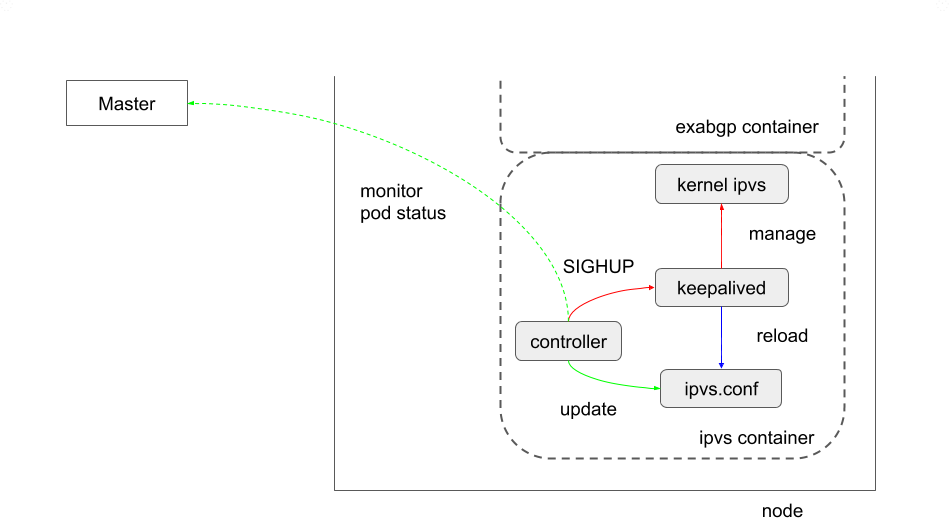
\includegraphics[width=\columnwidth]{Figs/ipvs-ingress-schem}
\caption{Implementation of ipvs container.}
The controller checks the pod status every second.
Upon a change of the status, the controller updates the ipvs.conf and sends SIGHUP to keepalived.
The keepalived updates the load balance table in the kernel correctly.
\label{fig:ipvs-ingress-schem}
\end{figure} 

The proposed load balancer needs to dynamically reconfigure the ipvs balancing rules whenever {\em pods} are created or deleted. 
Fig.~\ref{fig:ipvs-ingress-schem} is a schematic diagram of ipvs container to show the dynamic reconfiguration of the ipvs rules.
Two daemon programs, controller and keepalived, running in the container are illustrated.
The keepalived manages Linux kernel's ipvs rules depending on the ipvs.conf configuration file.
It can also periodically health check the liveness of a {\em real server}, 
which is represented as a combination of the IP addresses and port numbers of the target {\em pods}. 
If the health check to a {\em real server} fails, keepalived will remove that {\em real server} from the ipvs rules immediately.
\textcolor{blue}{
The interval of the health check is typically 1 to several seconds and is arbitrarily determined by users.  
}

\textcolor{blue}{
Every second, the controller monitors information concerning the running {\em pods} of a service in the Kubernetes cluster by consulting the apiserver running in the master through its API.
}
Whenever {\em pods} are created or deleted, the controller notices the change and automatically regenerate an appropriate ipvs.conf 
and issue SIGHUP to keepalived \textcolor{blue}{
within a second.}
Then, keepalived will reload the ipvs.conf, and modify the kernel's ipvs rules correctly depending on the result of the health check.

\textcolor{blue}{
When a pod is terminated, existing connections are reset by the node kernel.
The SYN packets sent to a pod after termination, but before the ipvs rule update, will be answered with ICMP unreachable by the node.
In these cases, the client sees connection errors.
In order to avoid the connection errors to be seen by a human, HTTP client programs are required to re-initiate the connection.
However, since the load balancer rule update is within a second, these errors can be regarded as the tolerable rare exceptions even without such re-initiations.
}

The actual controller\cite{ktaka_ccmp_2017_826894} is implemented using the Kubernetes ingress controller\cite{K8sIngress2017} framework. 
By importing existing Golang package, \enquote{k8s.io/ingress/core/pkg/ingress}, we could simplify the implementation, e.g. 
120 lines of code.  
%
Keepalived and the controller are placed in the docker image of ipvs container.
The ipvs is the kernel function and namespace separation for container has already been supported in the recent Linux kernel. 

Configurations for capabilities were needed when deploying the ipvs container: adding the CAP\_SYS\_MODULE capability 
to the container to allow the kernel to load required kernel modules inside a container, 
and adding CAP\_NET\_ADMIN capability to the container to allow keepalived to manipulate the kernel's ipvs rules. 
For the former case, we also needed to mount the \enquote{/lib/module} of the node's file system on the container's file system.

\subsection{BGP software container}

\begin{figure}[tb]

  \begin{subfigure}[t]{\columnwidth}
    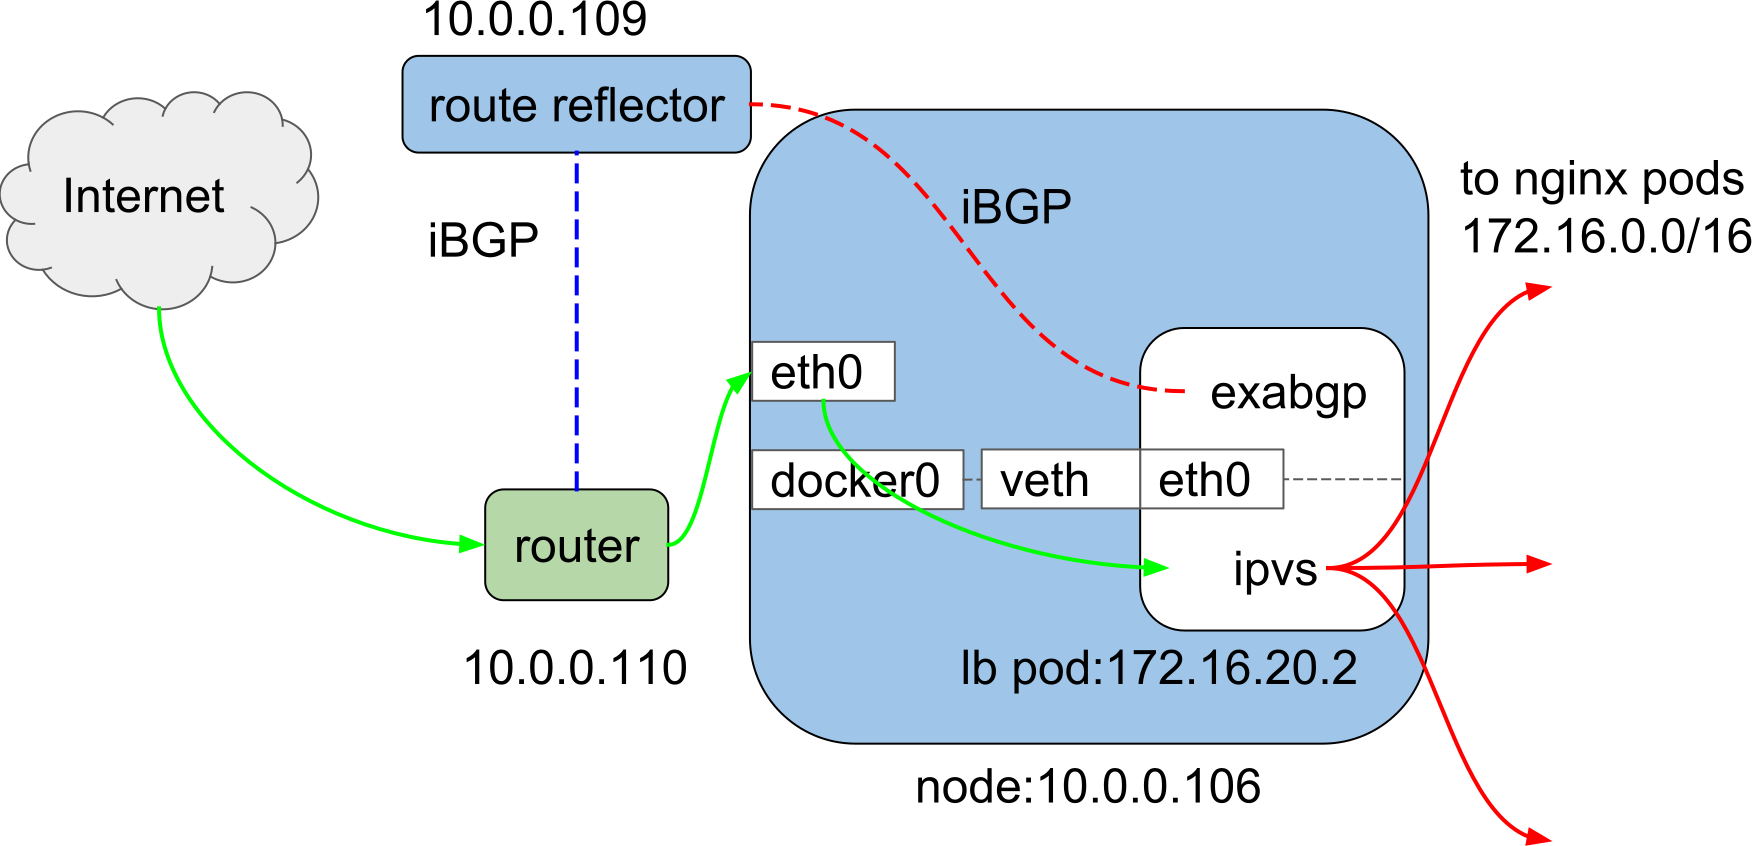
\includegraphics[width=0.9\columnwidth]{Figs/exabgp}
    \caption{}
    \label{fig:exabgp_schem}
  \end{subfigure}

  \par\bigskip

  \begin{subfigure}[t]{\columnwidth}

%\centering
\begin{Verbatim}[commandchars=\\\{\}]
───────────────────────────────────────────────────────
 [BGP announcement]
     route 10.1.1.0/24 next-hop 10.0.0.106       ...(1)

 [Routing in node net namespace]
     ip netns exec node \textbackslash
       ip route replace 10.1.1.0/24 dev docker0  ...(2)
      
 [Accept as local]
     ip route add local 10.1.1.0/24 dev eth0     ...(3)
───────────────────────────────────────────────────────
\end{Verbatim}
    \caption{}
    \label{fig:exabgp_setting}
  \end{subfigure}

  \caption{
    (a) Network path by the exabgp container.
%  For the green lines, a service IP address is used. The red lines use the IP addresses of the overlay network. The blue line uses the IP addresses of the node network.
    (b) Required settings in the exabgp container.
  }
\textcolor{blue}{
  (a): The packets from Internet to a service IP in 10.1.1.0/24 is routed to the load balancer pod(green arrows) by the set of routing rules shown in (b).
  And then the ipvs forwards them to IP addresses of nginx pods(red arrows).
  The IP address of any pod is dynamically assigned from 172.16.0.0/16 when the pod is started. 
  (b): (1)The node IP address, 10.0.0.106 is used as next-hop for the IP range 10.1.1.0/24 used by a service in BGP announcement.
  (2)In order to route the packets toward the IP used by the service to a container, a routing rule to the dev docker0 is created in the node net namespace.
  (3)A routing rule to accept the packets as local is also required. 
}
\label{fig:exabgp}
\end{figure}

In order to implement the ECMP redundancy, we also containerized exabgp using Docker.
Fig.\ref{fig:exabgp}~(\subref{fig:exabgp_schem}) shows a schematic diagram of the network path realized by the exabgp container.
We used exabgp as the BGP advertiser as mentioned earlier.
\textcolor{blue}{
The traffic from the Internet is forwarded by ECMP routing table on the router to the node that hosts a load balancer pod, then routed to that pod by the set of routing rules in Fig.\ref{fig:exabgp}~(\subref{fig:exabgp_setting}). 
And then the ipvs forwards them to IP addresses of nginx pods.
The IP address of any pod is dynamically assigned from 172.16.0.0/16 when the pod is started. 
}

Fig.\ref{fig:exabgp}~(\subref{fig:exabgp_setting}) summarises some key settings required for the exabgp container to route the traffic to the ipvs container.
In BGP announcements the node IP address, 10.0.0.106 is used as the next-hop for the IP range 10.1.1.0/24.
Then on the node, in order to route the packets toward 10.1.1.0/24 to the ipvs container, 
a routing rule to the dev docker0 is created in the node net namespace. 
A routing rule to accept the packets toward those IPs as local is also required in the container net namespace. 
A configuration for exabgp is shown in \ref{appendix:exabgp_config}.


\section{Evaluation}\label{Evaluation}

In order to verify the feasibility of the proposed load balancer architecture, we evaluated it with the following criteria;
(1) Basic functionality and Portability:
We evaluated the load balancer functionality using physical servers in on-premise data center and compared performance level with existing iptables DNAT and nginx as a load balancer.
We also carried out the same performance measurement in GCP and AWS to show the containerized ipvs load balancer is runnable even in the cloud environment.
(2) Redundancy and Scalability:
We evaluated ECMP functionality by watching routing table updates on the router when the new load balancer is added or removed.
We also evaluated the performance level by changing the number of load balancers.
%
The following subsections explain the evaluation in detail.

\subsection{Basic functionality and portability}

\begin{figure}[tb]

  \begin{subfigure}[t]{\columnwidth}
    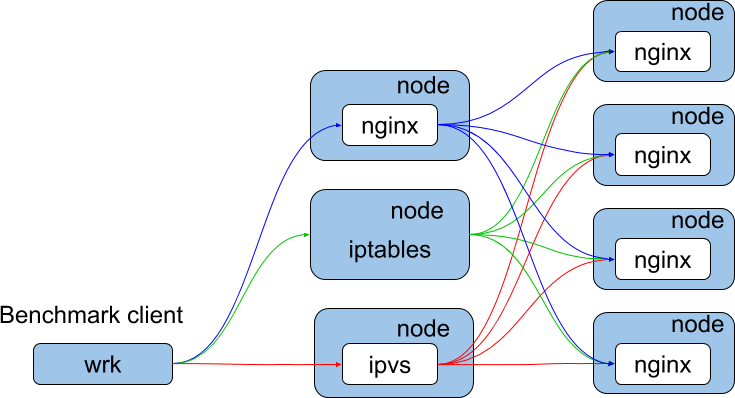
\includegraphics[width=0.9\columnwidth]{Figs/lb_single_schem}
    \caption{}
    \label{fig:lb_single_schem}
  \end{subfigure}

  \par\bigskip

  \begin{subfigure}[t]{\columnwidth}

\centering
\begin{Verbatim}[commandchars=\\\{\}]
───────────────────────────────────────────────────────
[Command line]
 wrk -c800 -t40 -d30s http://172.16.72.2:8888/
-c: concurrency, -t: # of thread, -d: duration

[Output example]
 Running 30s test @ http://10.254.0.10:81/
  40 threads and 800 connections
  Thread Stats   Avg      Stdev     Max   +/- Stdev
    Latency    15.82ms   41.45ms   1.90s    91.90%
    Req/Sec     4.14k   342.26     6.45k    69.24%
  4958000 requests in 30.10s, 1.14GB read
  Socket errors: connect 0, read 0, write 0, timeout 1
Requests/sec: 164717.63
Transfer/sec:     38.86MB
───────────────────────────────────────────────────────
\end{Verbatim}

    \caption{}
    \label{fig:bench_example}
  \end{subfigure}

  \caption{
    (a) Benchmark setup. (b) Benchmark command line and output example.
  }
  \label{fig:benchmark-schem}
\end{figure}


\begin{figure}[tb]

  \begin{subfigure}[t]{\columnwidth}
\begin{Verbatim}[commandchars=\\\{\}]
───────────────────────────────────────────────────────
[Hardware Specification in On-premise data center]
  CPU: Xeon E5-2450 2.10GHz 8 physical cores
  (with Hyper Threading) 
  Memory: 32GB
  NIC: Broadcom BCM5720 1Gbps
 (Node x 6, Load balancer x 1, Client x 1)

[GCP VM Instance Specification]
  Instance type: custom instance
  CPU: Xeon 2.2GHz, 8, 16, 32 cpus
  Memory: 16GB
  NIC: virtio_net /w 16 rx-queues, 1Gbps
 (Node x 6, Load balancer x 1, Client x 1)

[AWS VM Instance Specification]
  Instance type: c4.2xlarge, c4.4xlarge, c4.8xlarge 
  CPU: Xeon E5-2666 v3 2.90GHz, 8, 16, 32 cpus
  Memory: 64GB
  NIC: ixgbevf /w 2 rx-queues, 1Gbps
 (Node x 6, Load balancer x 1, Client x 1)
───────────────────────────────────────────────────────
\end{Verbatim}
    \caption{}
    \label{fig:machine_spec}
  \end{subfigure}

  \begin{subfigure}[t]{\columnwidth}
\begin{Verbatim}[commandchars=\\\{\}]
───────────────────────────────────────────────────────
[Node Software]
  OS: Debian 8.7, linux-3.16.0-4-amd64
  Kubernetes v1.10.6
  flannel v0.7.0
  etcd version: 3.0.15

[Container Software]
  Keepalived: v1.3.2 (12/03,2016)
  nginx : 1.11.1(load balancer), 1.13.0(web server) 
───────────────────────────────────────────────────────
\end{Verbatim}
    \caption{}
    \label{fig:software_spec}
  \end{subfigure}

  \caption{
    (a) Hardware and Virtual Machine specifications. (b)Software specifications.
  }
  \label{fig:benchmark-spec}
\end{figure}

\textcolor{blue}{
Throughput measurements were carried out in order to examine the basic functionality of the containerized ipvs load balancer.
Fig.~\ref{fig:benchmark-schem} shows the schematic diagram of the throughput measurement and the benchmark command line.
We measured the performance of the load balancers using a benchmark program called wrk\cite{Glozer2016}.
Multiple nginx {\em pods} are deployed on multiple nodes as web servers in the Kubernetes cluster.
In each nginx {\em pod}, single nginx web server that returns the IP address of the {\em pod} is running.
We then set up the ipvs, iptables DNAT, and nginx load balancers on one of the nodes, and performed the throughput measurement changing the number of the nginx pods.
The throughput is measured by sending out HTTP requests from the wrk towards a load balancer and by counting the number of responses the benchmark host received as shown in Fig.~\ref{fig:benchmark-schem}~(\subref{fig:lb_single_schem}).
}

\textcolor{blue}{
Fig.~\ref{fig:benchmark-schem}~(\subref{fig:bench_example}) shows an example of the command-line for wrk and the corresponding output.
The command-line in Fig.~\ref{fig:benchmark-schem}~(\subref{fig:bench_example}) will generate 40 wrk program threads
and allow those threads to send out a total of 800 concurrent HTTP requests over the period of 30 seconds.
The output example shows information including per-thread statistics, error counts, throughput in [Request/sec] and data rate in [Transfer/sec]
}

\textcolor{blue}{
Fig.~\ref{fig:benchmark-spec}~(\subref{fig:machine_spec}) shows hardware and virtual machine specifications for experiments in on-premise data center and cloud environments.
We used a total of eight servers; six servers for Nodes, one for the load balancer and one for the benchmark client, with all having the same hardware specifications.
The software versions used for Kubernetes, web server and load balancer {\em pods} used in our experiments are also summarized in Fig.~\ref{fig:benchmark-spec}~(\subref{fig:software_spec}).
}

\begin{figure}[h]

\begin{subfigure}[t]{\columnwidth}
  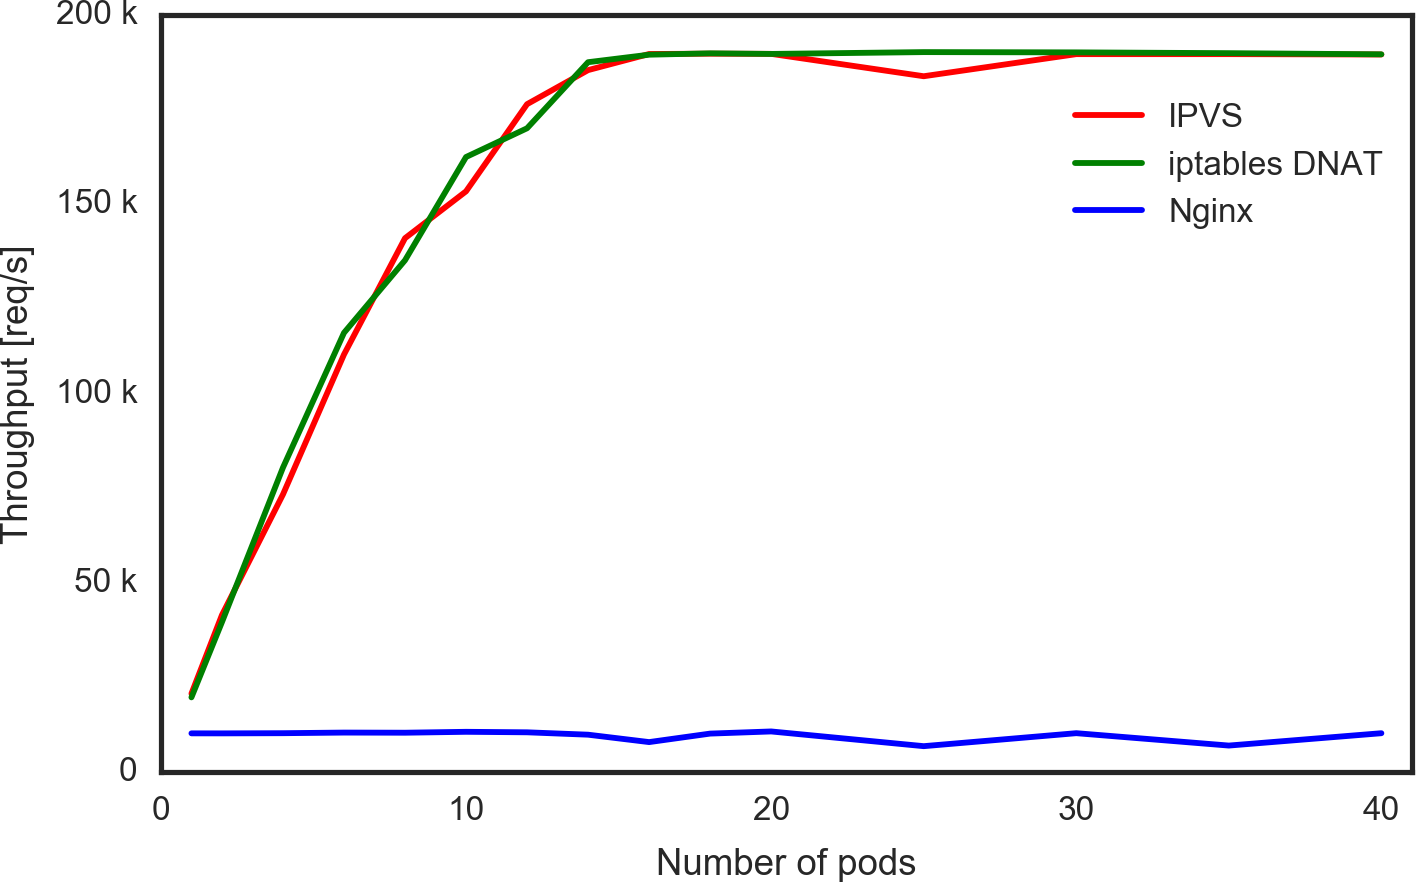
\includegraphics[width=0.9\columnwidth]{Figs/ipvs-iptables-nginx}
  \caption{On-premise data center.}
  \label{fig:ipvs-iptables-nginx}
\end{subfigure}

  \par\bigskip

  \begin{subfigure}[t]{\columnwidth}
    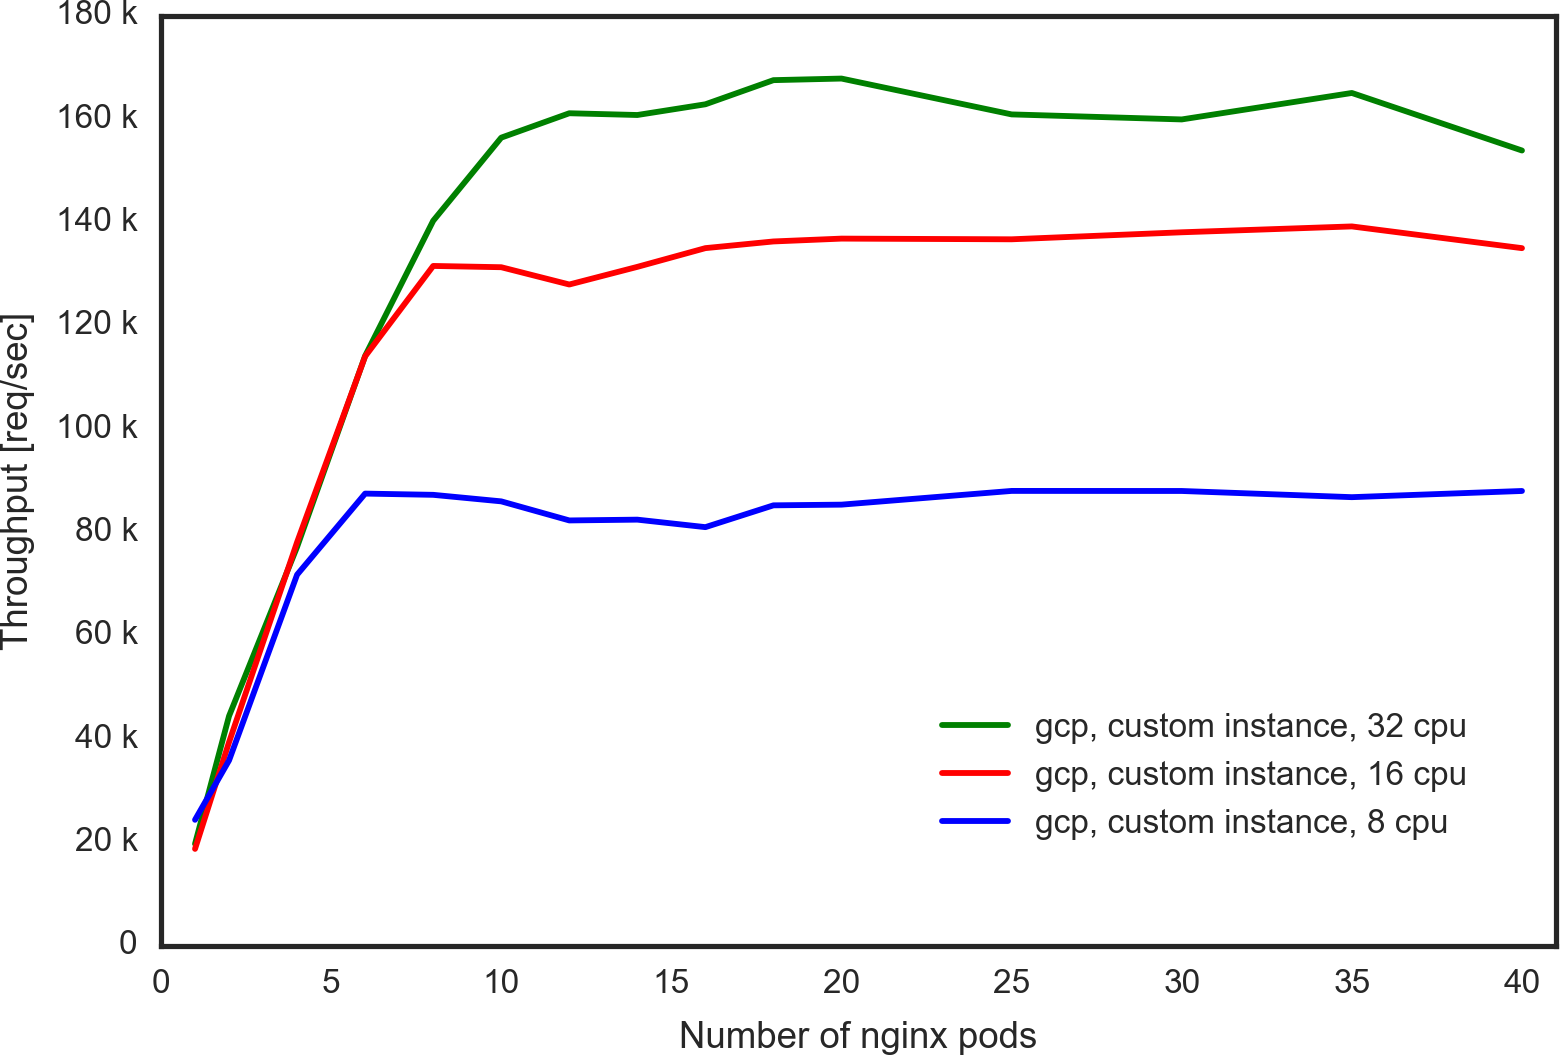
\includegraphics[width=0.9\columnwidth]{Figs/gcp_all_ieice}
    \caption{GCP.}
    \label{fig:gcp_all_ieice}
  \end{subfigure}

  \par\bigskip

  \begin{subfigure}[t]{\columnwidth}
    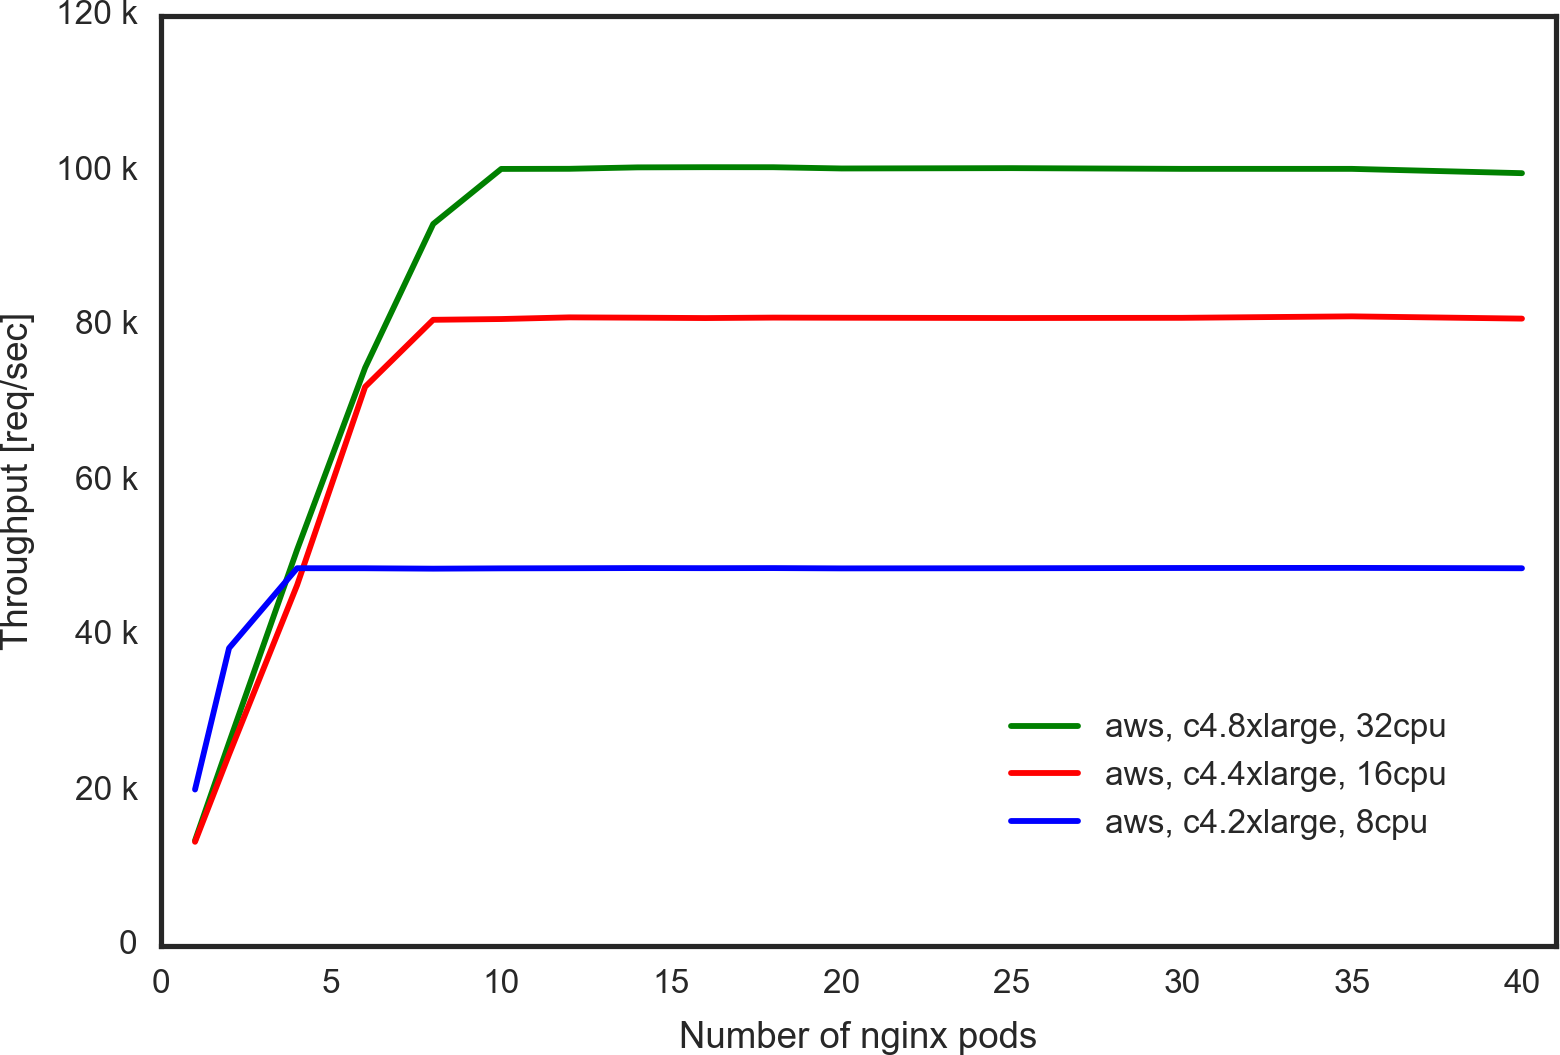
\includegraphics[width=0.9\columnwidth]{Figs/aws_c4_ieice}
    \caption{AWS.}
    \label{fig:aws_c4_ieice}
  \end{subfigure}

  \caption{Throughput measurement results of the proposed load balancer in on-premise data center(a), GCP(b), and AWS(c).
}
  \label{fig:ipvs_performance}

\end{figure}

\interfootnotelinepenalty=10000

Fig.~\ref{fig:ipvs_performance}~(\subref{fig:ipvs-iptables-nginx}) shows the throughput of the proposed ipvs container load balancer.
The performance of the nginx and the iptables DNAT as the load balancers are also presented for comparison.
As we increased the number of the nginx pods(web servers) from 1 to around 14, the throughput increased almost linearly and after which it saturated.
The increase indicates that the load balancer functions properly because it increased throughput by distributing HTTP requests to multiple of the web servers.
The saturated performance level indicates the maximum performance of the load balancer, which could be determined either by network bandwidth or CPU performance level of the load balancer or the benchmark client.
In this specific experiment, the performance level was limited by the 1 Gbps bandwidth of experimental network\cite{takahashi2018portable}, which is revealed by packet level analysis using tcpdump.\footnote{
On average the data size of each request and the corresponding response was in total about 636 [byte/req] including TCP/IP headers, Ethernet header, and inter frame gaps.
Multiplying that with 190K [req/sec] and 8 [bit/byte] will result in 966.72 Mbps.
}
While nginx did not show any benefit as the load balancer, the performance of the ipvs load balancer container showed equivalent performance level as the un-containerized iptables DNAT.
This means that our proposed ipvs container load balancer is at least as good as the un-containerized iptables' load balancing in the 1 Gbps network.

\textcolor{blue}{
Fig.~\ref{fig:ipvs_performance}~(\subref{fig:gcp_all_ieice}) and Fig.~\ref{fig:ipvs_performance}~(\subref{fig:aws_c4_ieice}) show the load balancer performance levels that are measured in GCP and AWS, respectively. In the case of GCP, custom instance with 32Gbyte memory and with 8, 16, and 32 CPU are used.
And in the case of AWS instance type of c4.2xlarge, c4.4xlarge, and c4.8xlarge are used.
These are aimed to show that our proposed load balancer can be run in cloud environments and also functions properly.
}

\textcolor{blue}{
Both results show similar characteristics as the experiment in an on-premise data center in Fig.~\ref{fig:ipvs_performance}~(\subref{fig:ipvs-iptables-nginx}), where throughput increased linearly to a certain saturation level that is determined by either network speed or machine specifications.
Since in the cases of cloud environments we can easily change the machine specifications, especially CPU counts, we measured throughput with several conditions of them.
From the first look of the results, since changing CPU counts changed the load balancer's throughput saturation levels, we thought VM's computation power limited the performance levels.
However, since there are cases in the cloud environment, where changing the VM types or CPU counts also changes the network bandwidth limit, a detailed analysis is further required in the future to clarify which factor limits the throughput in the cases of these cloud environments.
Still, we can say that the proposed ipvs load balancers can be run in GCP and AWS, and function properly.
}

\subsection{Redundancy and Scalability}

The ECMP technique is expected to make the load balancers redundant and scalable since all the load balancer containers act as active.
We examined the behavior of the ECMP routing table updates, by changing the number of the load balancers.
After that, in order to explore the scalability, we also measured the throughput from a benchmark client with ECMP routes when multiple of the ipvs container load balancers are deployed.

\begin{figure}[h]

\begin{subfigure}[b]{\columnwidth}
    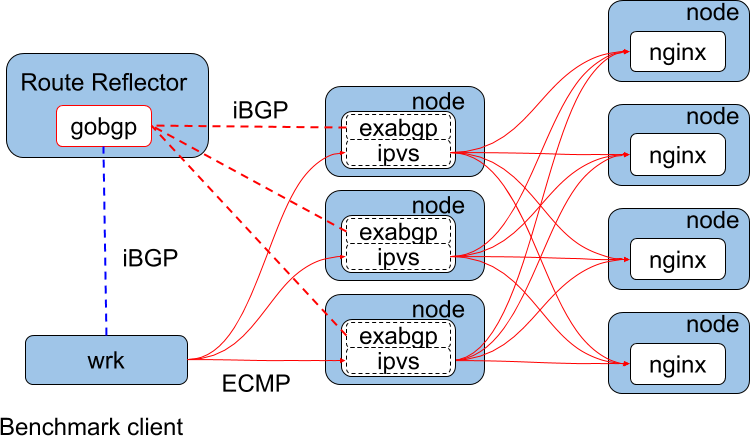
\includegraphics[width=0.9\columnwidth]{Figs/lb_ecmp_schem}
    \caption{}
    \label{fig:lb_ecmp_schem}
\end{subfigure}

  \begin{subfigure}[t]{\columnwidth}
\begin{Verbatim}[commandchars=\\\{\}]
───────────────────────────────────────────────────────
[Hardware Specification]
  CPU: Xeon E5-2450 2.10GHz 8 physical cores
  (with Hyper Threading) 
  Memory: 32GB
  NIC: Broadcom BCM5720 1Gbps
 (Node x 6, Load balancer x 4)

  CPU: Xeon E5-2450 2.10GHz 8 physical cores
  (with Hyper Threading) 
  Memory: 32GB
  NIC: Intel X550 10Gbps
 (Client x 1)
  
[Node Software]
  OS: Debian 9.5, linux-4.16.8
  Kubernetes v1.5.2
  flannel v0.7.0
  etcd version: 3.0.15

[Container Software]
  Keepalived: v1.3.2 (12/03,2016)
  nginx : 1.15.4(web server) 
───────────────────────────────────────────────────────
\end{Verbatim}
    \caption{}
    \label{fig:ecmp-hw_sw_spec}
  \end{subfigure}

  \caption{
    (a) Benchmark setup. (b) Hardware and software specifications.
  }
  \label{fig:ecmp-benchmark-schem}
\end{figure}

Fig.~\ref{fig:ecmp-benchmark-schem} shows the schematic diagram of the experimental setup and also summarizes hardware and software specifications.
Notable differences from the previous throughput experiment in Fig.~\ref{fig:benchmark-schem} are as follows;
1) Each load balancer pods now consists of both an ipvs container and an exabgp container.
2) The routing table of the benchmark client is updated by BGP protocol through a route reflector.
3) The NIC of the benchmark client has been changed to 10 Gbps card since now we have multiple of ipvs container load balancers that are capable of filling up 1 Gbps bandwidth.
4) Some of the software have been updated to the most recent versions at the time of the experiment.

\begin{figure}[h]

\begin{subfigure}[t]{\columnwidth}
\centering
\begin{Verbatim}[commandchars=\\\{\}]
───────────────────────────────────────────────────────
10.1.1.0/24 via 10.0.0.106 \textbackslash 
                        dev eth0 proto zebra metric 20
───────────────────────────────────────────────────────
\end{Verbatim}
\caption{Routing table entry with single load balancer pod.}
\label{fig:single}
\end{subfigure}
\par\bigskip

\begin{subfigure}[t]{\columnwidth}
\centering
\begin{Verbatim}[commandchars=\\\{\}]
───────────────────────────────────────────────────────
10.1.1.0/24 proto zebra metric 20
        nexthop via 10.0.0.105  dev eth0 weight 1
        nexthop via 10.0.0.106  dev eth0 weight 1
        nexthop via 10.0.0.107  dev eth0 weight 1
───────────────────────────────────────────────────────
\end{Verbatim}
\caption{Routing table entry with three load balancer pods.}
\label{fig:three}
\end{subfigure}
\par\bigskip

\begin{subfigure}[t]{\columnwidth}
\centering
\begin{Verbatim}[commandchars=\\\{\}]
───────────────────────────────────────────────────────
10.1.1.0/24 pro to zebra metric 20
        nexthop via 10.0.0.107  dev eth0 weight 1
        nexthop via 10.0.0.105  dev eth0 weight 1
        nexthop via 10.0.0.106  dev eth0 weight 1
10.1.2.0/24 proto zebra metric 20
        nexthop via 10.0.0.107  dev eth0 weight 1
        nexthop via 10.0.0.106  dev eth0 weight 1
───────────────────────────────────────────────────────
\end{Verbatim}
\caption{Routing table entry with two services with two and three load balancer pods respectively.}
\label{fig:double_svc}
\end{subfigure}
\par\bigskip

\caption{ECMP routing tables.}
\label{fig:exabgp_routing_table}
\end{figure}

First, we examined ECMP functionality by watching the routing table on the benchmark client.
Fig.~\ref{fig:exabgp_routing_table}~(\subref{fig:single}) shows the routing table entry on the router when a single load balancer pod exists.
From this entry, we can tell that packets toward 10.1.1.0/24 are forwarded to 10.0.0.106 where the load balancer pod is running.
It also shows that this routing rule is updated by zebra.

When the number of the load balancer pods is increased to three, we can see the routing table entry in Fig.~\ref{fig:exabgp_routing_table}~(\subref{fig:three}).
We have three next hops towards 10.1.1.0/24 each of which being the node where the load balancer pods are running.
The weights of the three next-hops are all 1.
The update of the routing entry was almost instant as we increased the number of the load balancers.

Fig.~\ref{fig:exabgp_routing_table}~(\subref{fig:double_svc}) shows the case where we additionally started new service with two load balancer pods with service addresses in 10.1.2.0/24 range.
We could accommodate two different services with different service IPs, one with three load balancers and the other with two load balancers on a group of nodes(10.0.0,105,10.0.0,106,10.0.0,107).
The update of the routing entry was almost instant as we started the load balancers for the second service.

\textcolor{blue}{
As far as the route withdrawal is concerned, if an exabgp is killed by SIGKILL or SIGTERM the kernel of the node close the BGP connection by sending out a packet with FIN flag to the peer gobgpd on the route reflector, and thus the route is withdrawn immediately.
The gobgp on the route reflector also periodically check the BGP connection, and if the peer exabgp container is unresponsive for more than the specified duration, “hold-time“ setting in gobgpd, it will also terminate the connection and withdraw the route.
The packets arriving within the duration will be dropped.
However, we can set up the “hold-time” short enough so that the retransmitted TCP packets from the client will be forwarded correctly to functioning load balancers.
}

\begin{figure}[t]

  \begin{subfigure}[t]{\columnwidth}
    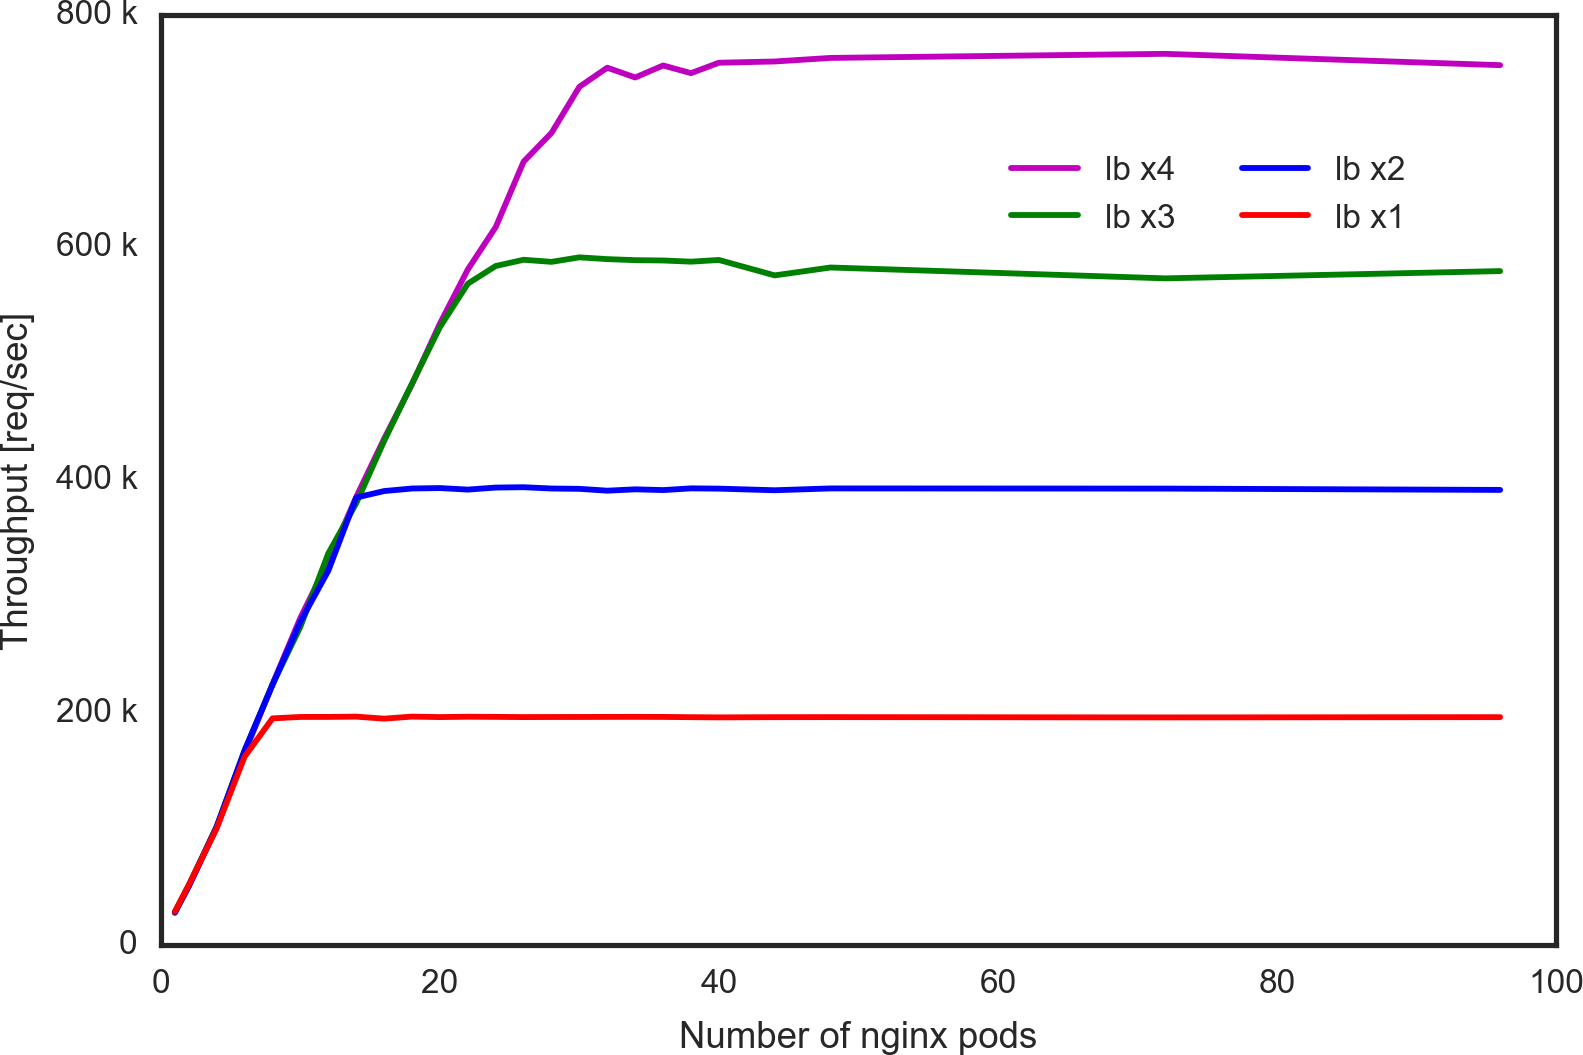
\includegraphics[width=0.9\columnwidth,left]{Figs/ecmp_lb_cubic_ieice}
    \caption{Throughput of ECMP redundant load balancer.}
    The throughputs are measured for a single load balancer(lb x1), two(lb x2), three(lb x3) and four(lb x4) load balancers.
    \label{fig:ecmp_lb_cubic_ieice}
  \end{subfigure}

  \par\bigskip

  \begin{subfigure}[t]{\columnwidth}
    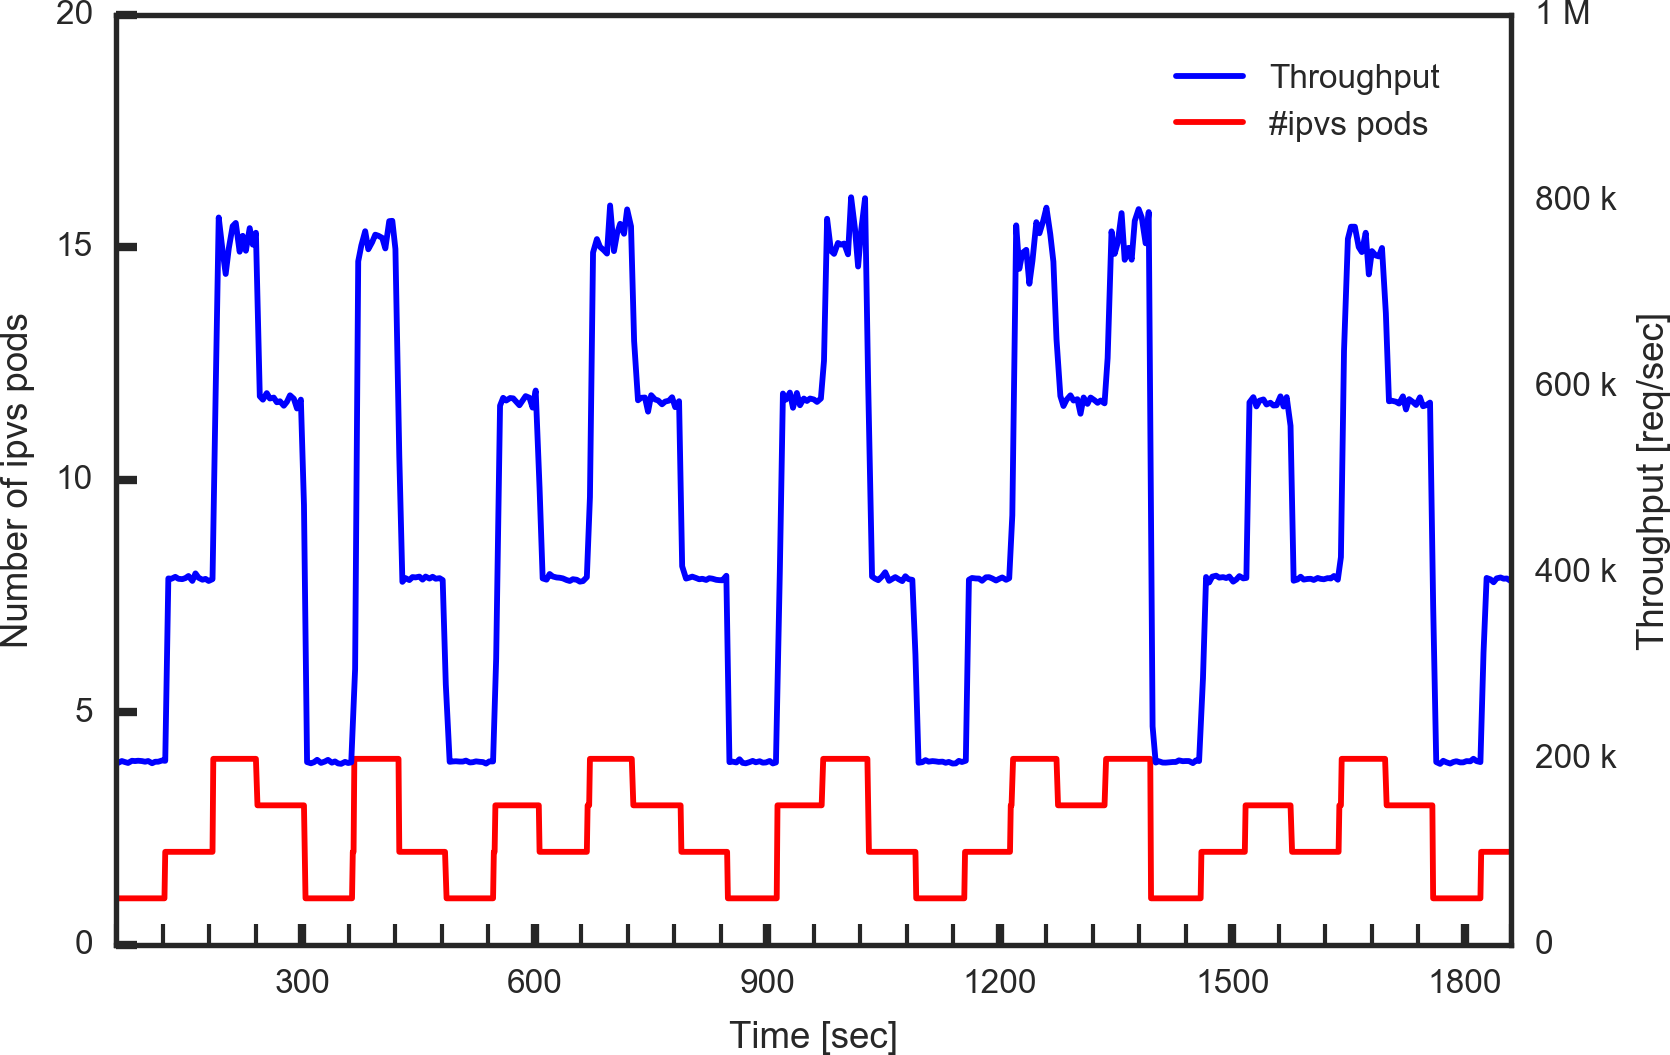
\includegraphics[width=0.98\columnwidth,left]{Figs/ecmp_response_ieice}
    \caption{Throughput responsiveness.}
    This shows the throughput responsiveness when the number of the load balancers was changed randomly in every 60 seconds.
    \label{fig:ecmp_response_ieice}
  \end{subfigure}

  \par\bigskip

  \begin{subfigure}[t]{\columnwidth}
    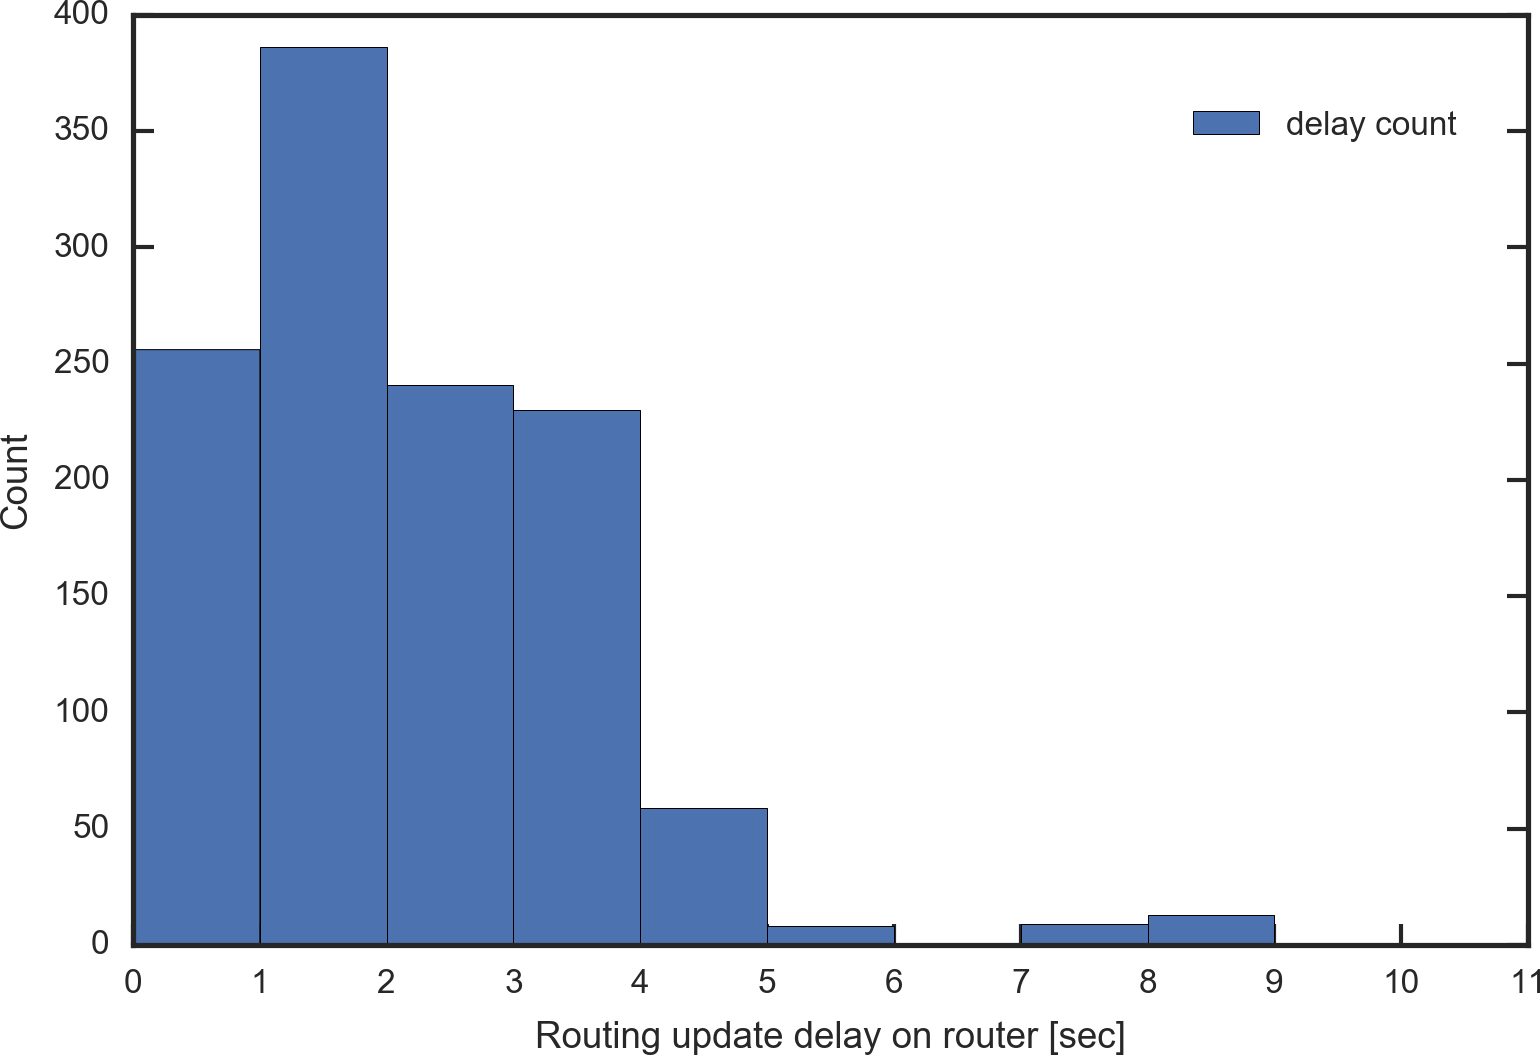
\includegraphics[width=0.9\columnwidth,left]{Figs/ecmp_delay_histgram_ieice}
  \caption{A histogram of the ECMP update delay.}
This shows the delays until the number of running ipvs pods is reflected into the routing table on the benchmark client,
when the number of the ipvs pods is changed randomly every 60 seconds for 20 hours.
    \label{fig:ecmp_delay_histgram_ieice}
  \end{subfigure}

  \caption{Scalability of portable load balancer with ECMP redundancy.}
  \label{fig:ecmp_scalability}

\end{figure}

\textcolor{blue}{
We also carried out throughput measurement to show that our proposed architecture increases the throughput as we increase the number of the load balancers.
Fig.~\ref{fig:ecmp_scalability}~(\subref{fig:ecmp_lb_cubic_ieice}) shows the results of the measurements.
There are four solid lines in the figure, each corresponding the throughput result when there are one through four of the proposed load balancers.
The saturated levels, i.e. performance levels depend on the number of the ipvs load balancer pods(lb x 1 being the case with one ipvs pods, and lb x2 being two of them and as such). The performance level increases linearly as we increases the number of the load balancers up to four of the ipvs load balancers, but did not scale further.
This was because we used up CPU power of the benchmark client since the CPU usage was 100\% when there were more than four load balancers.
We expect that replacing the benchmark client with more powerful machines, or changing the experimental setup so that multiple benchmark clients can access the load balancers through an ECMP router, will improve the performance level further.
}

\textcolor{blue}{
Fig.~\ref{fig:ecmp_scalability}~(\subref{fig:ecmp_response_ieice}) shows the throughput measurement results when we periodically changed the number of the load balancers. 
The red line in the figure shows the number of the ipvs load balancer pods, which we changed randomly every 60 seconds.
The blue line corresponds to the resulting throughput.
As we can see from the figure, the blue line nicely follows the shape of the red line.
This indicates that new load balancers are immediately utilized after they are created, and after removing some load balancers, the traffic to them is immediately directed to the existing load balancers.
}

\textcolor{blue}{
Fig.~\ref{fig:ecmp_scalability}~(\subref{fig:ecmp_delay_histgram_ieice}) shows histogram of the ECMP update delay, where we measured the delays until the number of running ipvs pods is reflected in the routing table on the benchmark client, as we change the number of the ipvs pods randomly every 60 seconds for 20 hours.
As we can see from the figure, most of the delays are within 6 seconds, and the largest delay during the 20 hours experiment was 10 seconds.
We can conclude that ECMP routing update in our proposed architecture is quick enough.
}

\FloatBarrier

\subsection{Resource Consumption}

\textcolor{blue}{
Fig.~\ref{fig:cpu_usage} compares the CPU usage for proposed load balancer(ipvs in a container) and iptables DNAT at the time of the throughput measurement in the on-premise data center.
Since the CPU usage was higher for the ipvs in a container, the proposed load balancer may be less efficient compared with the iptables DNAT.
%The proposed architecture requires additional computational resources compared with the conventional architecture.
However since single hardware can accommodate 1 Gbps traffic with CPU usage of about 60\%, the authors regard this as a tolerable overhead.
The authors plan to improve the efficiency of the proposed load balancer by developing a software load balancer using eXpress data path(XDP) technology\cite{hoiland2018express} in the future work and thereby improving the performance levels of the portable load balancer.
}

\begin{figure}[h]
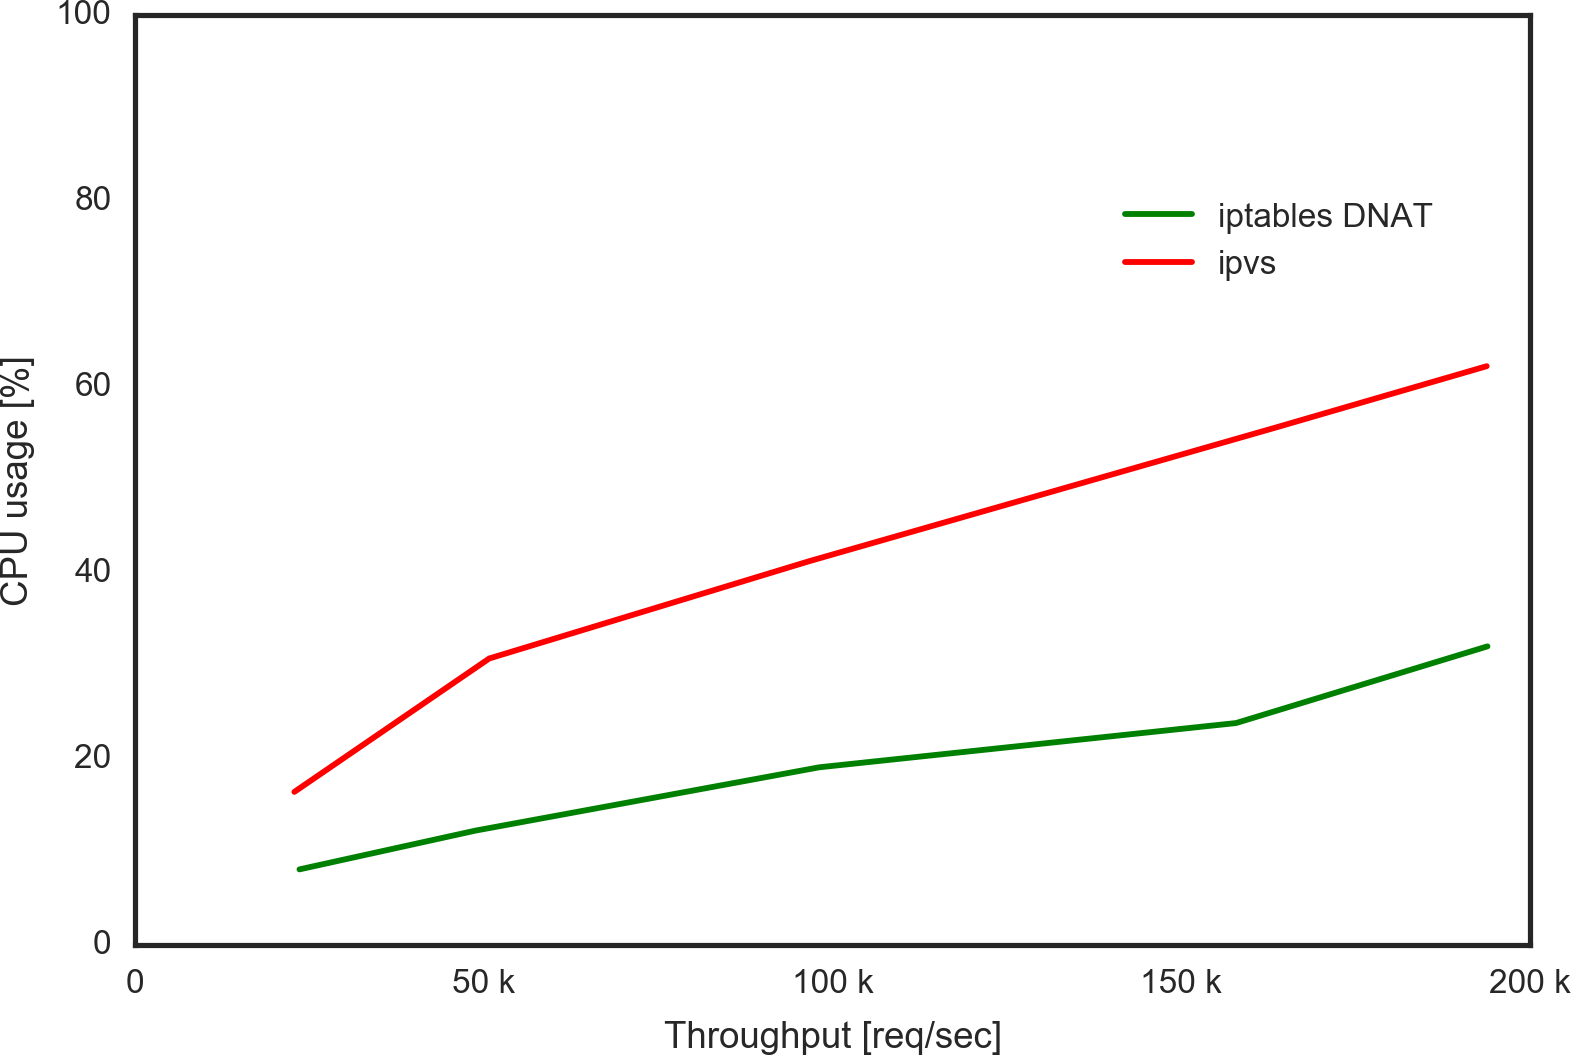
\includegraphics[width=\columnwidth]{Figs/cpu_usage}
\caption{CPU usage of the ipvs and iptables DNAT.}
\label{fig:cpu_usage}
\end{figure}

\section{Conclusions}\label{Conclusions}

In this paper, we proposed a portable load balancer with ECMP redundancy for the Kubernetes cluster systems that is aimed at facilitating migration of container clusters for web services.
We implemented an experimental web cluster system with multiple of load balancers and web servers using Kubernetes and OSSs on top of standard Linux boxes to prove the functionality of the proposed architecture.
We conducted performance measurements and found that the ipvs based load balancer in container functioned properly both in on-premise data center and cloud environments while it showed the comparable performance levels as the existing iptables DNAT based load balancer.
We also carried out experiments to verify the feasibility of ECMP redundancy in on-premise data center, and revealed that it functions properly with linear scalability up to four load balancers.

The current limitations of this study are;
1) Currently, BGP peering is not supported in GCP and AWS, and thus redundancy is achieved only by route update through cloud API upon the start of a load balancer.
The authors expect the cloud providers to support it in the future.
2) Most of the experiments are in 1Gbps network environments.
For future work, we plan to carry out throughput measurement in 10Gbps network environments and also improve the performance of a single software load balancer on standard Linux box using XDP technology.

